\documentclass[11pt,twocolumn]{article}
\title{Final Project: Face detector}
\author{Brendan Miller}
\date{March 12 2012}
\usepackage{multirow,amsmath}
\usepackage{graphicx}
\usepackage{fancyvrb}
\usepackage{color}
\usepackage{amsfonts}
\usepackage{hyperref}
\begin{document}
\twocolumn[
\begin{@twocolumnfalse}
\maketitle
\begin{abstract}
A face detector implemented via a simplified Viola Jones algorithm.
\end{abstract}
\end{@twocolumnfalse}
]

\section{Project Overview}

For this project I implemented an binary image classifier that detects
faces. This is based on the work of Paul Viola and Michael
Jones\cite{violajones2001}.

Features are extracted from images by first generating what they
termed Viola and Jones termed an integrated image. From the integrated
image, a large number of real valued features, described more fully in
the section \ref{sec:features} are rapidly computed.

Given a large set of real valued features, a weak learner is
constructed by selecting a single feature and a threshhold value that
partitions example images into guessed face and non-face classes. This
weak learner is conceptually similar to a decision tree stump,
although the metric used to find the optimal feature and threshold
is different (see section \ref{sec:weaklearner}).

Weak learners are combined with boosting (see section
\ref{sec:boosting}) in order to increase accuracy.

Finally, in the original Viola Jones paper, boosted classifiers were
combined in a cascade. The cascade was designed to reduce the
incendence of false positives, and to increase the performance of the
final classifer and possibly of the training phase. For my project I
have ommitted the cascade, as I said I would in my original project
proposal.

Even without the cascade, I've managed to achieve very high accuracy,
upwards of 99\%\footnote{Note this is on a validation set selected
  from the images provided with the project. I would expect accuracy
  to drop on images from a less carefully curated source.}, using a
boosted classifier over the features described in the original Viola
Jones paper.

\section{Feature Extraction}
\label{sec:features}

\begin{figure}
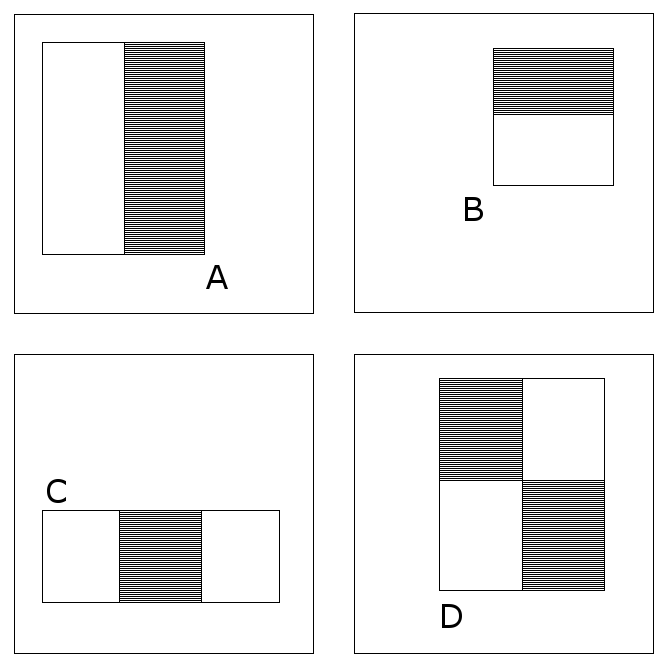
\includegraphics[width=40mm]{features.png}
\caption{Image features used to train the weak learner. Image from wikipedia.}
\label{fig:features}
\end{figure}

The underlying features used to train the weak classifier are
illustrated in figure \ref{fig:features}. These rectangular features are computed by summing
values of the pixels under the greyed out section, and subtracting the
sum of the pixels under the white section to produce a real valued
feature. For each feature type, a feature for every possible scale and
translation over the image are computed.

Rapid computation of these features probably the most important
innovation in Viola Jones. As discussed in the Viola Jones
algorithm\cite{violajones2001}, other detectors provide similar levels of
accuracy, but Viola Jones provides greatly improved performance.

To rapidly classify images, and also to provide more reasonable
training speeds, the features discussed in this paper can be quickly
computed by first creating an integral image. The integral image is of
the same dimension of the source image, but every element of the
integral image is the sum of all pixels above and to the left of that
coordinate in the source image.

From this integral image, the sum of a rectangular area can be
computer with only 4 array references, one to each corner of the
rectangle. A little algebra will similarly allow features A, B, C, and
D to be computed with a small number of references.

Even using the integrated image, the performance of feature
computation can be a drag on the algorithm. Especially in training on
large datasets, when millions of features need to be computed, it is
extremely important that feature computation is fast. For this reason,
after finding my initial pure python implementation to be too slow, I
rewrote the feature extraction code in C++, which made training go
about 5 times faster.

Another optimization that benefits the speed of training, but not of
classification, is to precompute all features and store them in main
memory. Originally I implemented my training stage this way, but found
that on large datasets the number of precomputed features was too
large to fit in main memory on a 32 bit machine.

For a 16 by 16 image, in my implementation there are 26944
features. Given 6000 training examples and 4 bytes per feature,
roughly 154 gigabytes of memory are necessary to precompute all the
features. Currently this is not practical.

\section{Weak Learner}
\label{sec:weaklearner}

The weak learner used in the Viola Jones algorithm is very similar to
a stump decision tree classifier. The primary difference is that while
a stump classifier chooses a partition that maximizes weighted
information gain, the weak learner minimizes weighted
misclassification error.

\begin{align*}
  w_i = \mbox{weight of example $i$}\\
  h(x) = \mbox{weak learner classifier}\\
  \sum_i w_i |h(x_i) - y_i|
\end{align*}

This metric is important for performance reasons.

If for each feature we consider all threshold mid way between the
unique values of the feature in sorted order, then for $K$ features and
$N$ examples there are $K (N - 1)$ feature threshold combinations.

Sorting the examples by each of the features in turn takes $O(n m
\log(m))$ time.

For each feature assuming the examples are already sorted, the
threshold that minimizes weighted misclassification can be found in
linear time with respect to $N$ using a simple algorithm described in
Robust Real Time Face Detection\cite{violajones2004}. Finding the
minimal misclassification threshold for each $K$ features is thus a
$O(N K)$ operation.

TODO: current implementation does this in $O(K N \log(N))$ make a note
of that or fix it.

Comparatively, calculating the information gain of an individual
partition is a linear time operation with respect to the number of
examples $N$. Since that operation needs to be performed $N - 1$ times
for each of the $K$ features, training a weak classifier using
information gain as a metric would take $O(n m^2)$ time.

\section{Boosted Classifier}
\label{sec:boosting}

The weak learners are combined in a fairly standard boosting algorithm
as described by Schapire\cite{schapire2001}.

TODO: fill this out or remove the section.

\section{Experimental Results}

My training data\cite{trainingdata} is provided with my project and consists of 3000
images of faces and 10000 images of non-faces. All are 16 X 16
grayscale images.

Using 50 rounds of boosting and 5000 randomly selected training
images, I produced a classifier\footnote{This classifier is serialized
  as JSON in the file large\_classifier.json.}  that accurately
classifies faces over a validation set of 1000 images with 0.7\%
error. It produced 5 false positives and 2 false negatives.

Classification by this classifier is relatively rapid. Once the
integrated images have been generated, classification of 6000 images
took place in 1180 milliseconds using the C++ backend\footnote{By
  comparison the python backend took 9615 milliseconds.}. Thus it
takes about 0.2 milliseconds to classify an image. Note that in
practice the classifier would be run many times over a single image at
different scales and translations in order to detect faces at
different locations.

\begin{figure}
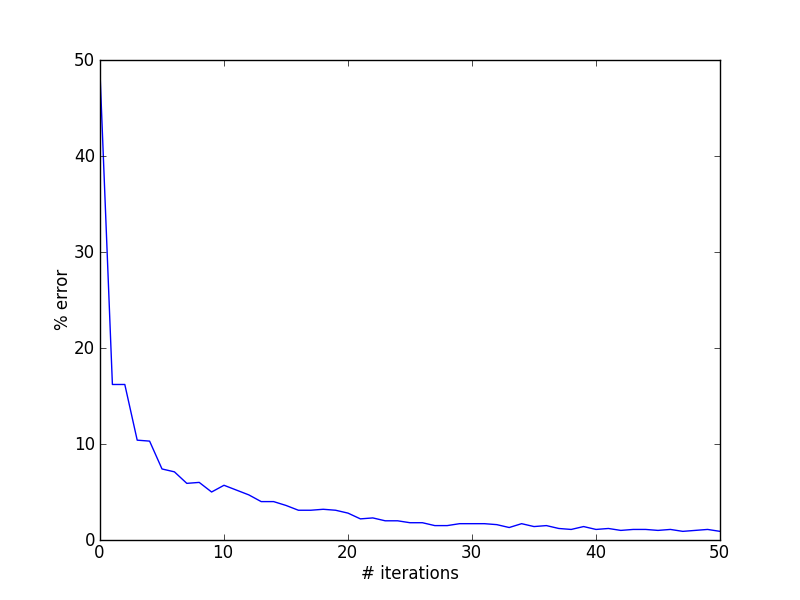
\includegraphics[width=60mm]{pct_err.png}
\caption{Percent error over 6000 images given rounds of boosting.}
\label{fig:bootingiter}
\end{figure}


\section{Future Directions}

Training of weak learners is fairly parallelizable using fork join
parallelism. 

\begin{thebibliography}{9}

\bibitem{violajones2001}
  Paul Viola, Michael Jones\\
  Rapid Object Detection using a Boosted Cascade of Simple Features\\
  \url{http://research.microsoft.com/en-us/um/people/viola/Pubs/Detect/violaJones_CVPR2001.pdf}

\bibitem{violajones2004}
  Paul Viola, Michael Jones\\
  Robust Real Time Face Detection\\
  \url{http://www.vision.caltech.edu/html-files/EE148-2005-Spring/pprs/viola04ijcv.pdf}

\bibitem{schapire2001}
  Robert E. Schapire\\
  The Boosting Approach to Machine Learning: An Overview\\
  \url{http://www.cs.princeton.edu/~schapire/uncompress-papers.cgi/msri.ps}

\bibitem{trainingdata}
  Training data used for my project\\
  \url{http://www.stat.ucla.edu/~yuille/courses/Stat231-Fall08/}

\end{thebibliography}



\end{document}